\chapter{Results}
\label{chap:Results}
\section{Time Invariant Simulation Results}
In this section I will be covering my results for the time-invariant model %
as described in chapter \ref{chap:System}. The results will be broken %
down into two sections, first we will examine the LMS algorithm and %
its convergence, then we will examine the NLMS algorithm.

\subsection{Least Mean Square}
\FloatBarrier
The three key measures of the LMS algorithm are it's mean square error, %
mean square deviation, and excess mean square error. %
The mean square error is a measure of how close the estimate is to the %
desired output and is defined as 
\begin{align}
	J = E\left[ \lvert d(n) - y(n) \rvert^{2} \right]
\end{align}
Mean square deviation is a measure of how much error there is %
between the optimal filter coefficients and the estimated %
channel coefficients and is defined as
\begin{align}
	\mathscr{D} = E\left[ \lvert w_{o}(n) - \hat{w}(n) \rvert^{2} \right]
\end{align}
And the excess mean square error is a measure of how much %
difference there is between the mean square error of the %
optimal solution and the estimated solution and is defined as
\begin{align}
	J_{\text{excess}} = J_{o} - J
\end{align}
Figures \ref{fig:LMS-MSE}, \ref{fig:LMS-MSD}, and \ref{fig:LMS-EMSE} %
show the results for mean square error, mean square deviation and %
excess mean square error for the LMS filter under a variety of %
different step sizes $\mu$.
\begin{figure}[ht]
	\centering
	\begin{minipage}{0.49\textwidth}
		\centering
		\includegraphics[width=\linewidth]{./Figures/Results/%
		TimeInvariantLMS/NoDivergence/ExcessMeanSquareError.png}
		\caption{Excess Mean Square Error of LMS}
		\label{fig:LMS-EMSE}
	\end{minipage}
	\begin{minipage}{0.49\textwidth}
		\centering
		\includegraphics[width=\linewidth]{./Figures/Results/%
		TimeInvariantLMS/NoDivergence/MeanSquareDeviation.png}
		\caption{Mean Square Deviation of LMS}
		\label{fig:LMS-MSD}
	\end{minipage}
\end{figure}
\begin{figure}[ht]
	\centering
	\includegraphics[width=0.55\textwidth]{./Figures/Results/%
	TimeInvariantLMS/NoDivergence/MeanSquareError.png}
	\caption{Mean Square Error of LMS}
	\label{fig:LMS-MSE}
\end{figure}
It's apparent for the figures that as the step size increases the %
rate of convergence increases as well. Recalling the discussion in %
chapter \ref{chap:AdaptiveFiltering} on adaptive filtering, this agrees %
with the intuition of larger step sizes moving more quickly down the error %
surface towards the optimum solution. Drawing our attention to figure %
\ref{fig:LMS-EMSE} it's clear that for larger step sizes the excess %
mean square error is higher in steady state. This also agrees with the %
stochastic gradient theory. When the step size is large, noise will cause %
the LMS filter to overshoot the optimum solution and oscillate around it, %
leading to larger excess mean square error or misadjustment. This confirms %
that given the time invariant system model the LMS filter operating in the %
frequency domain does in fact converge to the optimal solution and that %
the expected tradeoff between convergence time and misadjustment is %
present.
\begin{figure}[ht]
	\centering
	\begin{minipage}{0.49\textwidth}
		\includegraphics[width=\linewidth]{./Figures/Results/%
		TimeInvariantLMS/Divergence/MeanSquareDeviation.png}
		\caption{Mean Square Deviation diverging of LMS}
		\label{fig:LMS-MSD-Diverge}
	\end{minipage}
	\begin{minipage}{0.49\textwidth}
		\includegraphics[width=\linewidth]{./Figures/Results/%
		TimeInvariantLMS/Divergence/ExcessMeanSquareError.png}
		\caption{Excess Mean Square Error diverging of LMS}
		\label{fig:LMS-EMSE-Diverge}
	\end{minipage}
\end{figure}
\begin{figure}[ht]
	\centering
	\includegraphics[width=0.55\textwidth]{./Figures/Results/%
	TimeInvariantLMS/Divergence/MeanSquareError.png}
	\caption{Mean Square Error diverging of LMS}
	\label{fig:LMS-MSE-Diverge}
\end{figure}
Table \ref{tab:LMS} lists that valid step sizes for $\mu$ range between %
$0$ and $2/(M S_{\text{max}})$, however this is only valid for when %
$M$ is large. Instead we will examine the divergence of the LMS filter %
under the condition that $\mu$ must be between:
\begin{align}
	0 < \mu < \frac{2}{\sigma^{2}}
	\label{eq:LMS-Stability}
\end{align}
Where $\sigma^{2}$ is the variance in the input signal, and can also %
be thought of as the average power of the input signal. This follows %
directly from the conditions imposed upon step size by the gradient %
descent optimisation method. Figures \ref{fig:LMS-MSE-Diverge}, %
\ref{fig:LMS-MSD-Diverge}, \ref{fig:LMS-EMSE-Diverge} are %
show systems that diverge at a $\mu = 0.35$. This occurs %
when the randomly generated fading is very large and reduces %
the upper bound in equation \ref{eq:LMS-Stability} to beneath %
$\mu$.
\FloatBarrier
\subsection{Normalized Least Mean Square}
\FloatBarrier
Similarly to the LMS filter the NLMS filter also demonstrates convergence %
to the optimal solution as can be seen in figures \ref{fig:NLMS-MSE}, %
\ref{fig:NLMS-MSD}, and \ref{fig:NLMS-EMSE}. It's very apparent when %
comparing the $\mu = 0.05$ lines of the LMS and NLMS filters that the %
NLMS filter has faster convergence. The NLMS filter also has a greater range of %
convergent choices for $\mu$ as can be seen from the legend. This is an agreement %
with equation \ref{eq:SayedNLMSBound}. At higher choices of $\mu$ the NLMS also has %
a much higher misadjustment as can be seen in figure \ref{fig:NLMS-EMSE} which is %
a result of the faster rate of convergence. The regularisation parameter chosen %
for this NLMS experiment is chosen to be $0.05$.
\begin{figure}[ht]
	\centering
	\begin{minipage}{0.49\textwidth}
		\includegraphics[width=\linewidth]{./Figures/Results/%
		TimeInvariantNLMS/NoDivergence/MeanSquareDeviation.png}
		\caption{Mean Square Deviation of NLMS}
		\label{fig:NLMS-MSD}
	\end{minipage}
	\begin{minipage}{0.49\textwidth}
		\includegraphics[width=\linewidth]{./Figures/Results/%
		TimeInvariantNLMS/NoDivergence/ExcessMeanSquareError.png}
		\caption{Excess Mean Square Deviation of NLMS}
		\label{fig:NLMS-EMSE}
	\end{minipage}
\end{figure}
\begin{figure}[ht]
	\centering
	\includegraphics[width=0.55\textwidth]{./Figures/Results/%
	TimeInvariantNLMS/NoDivergence/MeanSquareError.png}
	\caption{Mean Square Error of NLMS}
	\label{fig:NLMS-MSE}
\end{figure}
In figures \ref{fig:NLMS-MSE-Diverge}, \ref{fig:NLMS-MSD-Diverge}, and %
\ref{fig:NLMS-EMSE-Diverge} it's apparent that for choices of $\mu$ greater %
than $2$ the NLMS algorithm diverges.
\begin{figure}[ht]
	\centering
	\begin{minipage}{0.49\textwidth}
		\centering
		\includegraphics[width=\linewidth]{./Figures/Results/%
		TimeInvariantNLMS/Divergence/MeanSquareDeviation.png}
		\caption{Mean Square Deviation Divergence of NLMS}
		\label{fig:NLMS-MSD-Diverge}
	\end{minipage}
	\begin{minipage}{0.49\textwidth}
		\centering
		\includegraphics[width=\linewidth]{./Figures/Results/%
		TimeInvariantNLMS/Divergence/ExcessMeanSquareError.png}
		\caption{Excess Mean Square Error Divergence of NLMS}
		\label{fig:NLMS-EMSE-Diverge}
	\end{minipage}
\end{figure}
\begin{figure}[ht]
	\centering
	\includegraphics[width=0.55\textwidth]{./Figures/Results/%
	TimeInvariantNLMS/Divergence/MeanSquareError.png}
	\caption{Mean Square Error Divergence of NLMS}
	\label{fig:NLMS-MSE-Diverge}
\end{figure}

\section{Time Varying Simulation Results}
\label{sec:TVResults}
\begin{figure}[ht]
	\includegraphics[width=\textwidth]{./Figures/Results/%
LMS_Time_Varying/LongCP/DD/HighSNR/LongTimeCoherence/%
MeanSquareError.png}
	\caption{Mean Square Error of Time Varying LMS with 
	a long cyclic prefix, in decision directed operation, with 
	a long coherence time at high SNR}
\end{figure}
\begin{figure}[ht]
	\includegraphics[width=\textwidth]{./Figures/Results/%
LMS_Time_Varying/LongCP/DD/HighSNR/MediumTimeCoherence/%
MeanSquareError.png}
	\caption{Mean square error of time varying LMS with a 
	long cyclic prefix, in decision directed operation, with a 
	medium coherence time at high SNR}
	\label{fig:Medium-High-Directed-Long}
\end{figure}
\begin{figure}[ht]
	\includegraphics[width=\textwidth]{./Figures/Results/%
LMS_Time_Varying/LongCP/DD/HighSNR/ShortTimeCoherence/%
MeanSquareError.png}
	\caption{Mean square error of time varying LMS with a 
	long cyclic prefix, in decision directed operation, with a 
	short coherence time at high SNR}
\end{figure}
\begin{figure}[ht]
	\includegraphics[width=\textwidth]{./Figures/Results/%
LMS_Time_Varying/LongCP/DD/LowSNR/LongTimeCoherence/%
MeanSquareError.png}
	\caption{Mean square error of time varying LMS with a 
	long cyclic prefix, in decision directed operation, with a 
	long coherence time at low SNR}
\end{figure}
\begin{figure}[ht]
	\includegraphics[width=\textwidth]{./Figures/Results/%
LMS_Time_Varying/LongCP/DD/LowSNR/MediumTimeCoherence/%
MeanSquareError.png}
	\caption{Mean square error of time varying LMS with a 
	long cyclic prefix, in decision directed operation, with a 
	medium coherence time at low SNR}
\end{figure}
\begin{figure}[ht]
	\includegraphics[width=\textwidth]{./Figures/Results/%
LMS_Time_Varying/LongCP/DD/LowSNR/ShortTimeCoherence/%
MeanSquareError.png}
	\caption{Mean square error of time varying LMS with a 
	long cyclic prefix, in decision directed operation, with a 
	short coherence time at low SNR}
\end{figure}
\begin{figure}[ht]
	\includegraphics[width=\textwidth]{./Figures/Results/%
LMS_Time_Varying/LongCP/NoDD/HighSNR/LongTimeCoherence/%
MeanSquareError.png}
	\caption{Mean square error of time varying LMS with a 
	long cyclic prefix, with a long coherence time at high SNR}
\end{figure}
\begin{figure}[ht]
	\includegraphics[width=\textwidth]{./Figures/Results/%
LMS_Time_Varying/LongCP/NoDD/HighSNR/MediumTimeCoherence/%
MeanSquareError.png}
	\caption{Mean square error of time varying LMS with a 
	long cyclic prefix, with a medium coherence time at high SNR}
\end{figure}
\begin{figure}[ht]
	\includegraphics[width=\textwidth]{./Figures/Results/%
LMS_Time_Varying/LongCP/NoDD/HighSNR/ShortTimeCoherence/%
MeanSquareError.png}
	\caption{Mean square error of time varying LMS with a 
	long cyclic prefix, with a short coherence time at high SNR}
	\label{fig:LMS-Short-High-None}
\end{figure}
\begin{figure}[ht]
	\includegraphics[width=\textwidth]{./Figures/Results/%
LMS_Time_Varying/LongCP/NoDD/LowSNR/LongTimeCoherence/%
MeanSquareError.png}
	\caption{Mean square error of time varying LMS with a 
	long cyclic prefix, with a long coherence time at low SNR}
\end{figure}
\begin{figure}[ht]
	\includegraphics[width=\textwidth]{./Figures/Results/%
LMS_Time_Varying/LongCP/NoDD/LowSNR/MediumTimeCoherence/%
MeanSquareError.png}
	\caption{Mean square error of time varying LMS with a 
	long cyclic prefix, with a medium coherence time at low SNR}
\end{figure}
\begin{figure}[ht]
	\includegraphics[width=\textwidth]{./Figures/Results/%
LMS_Time_Varying/LongCP/NoDD/LowSNR/ShortTimeCoherence/%
MeanSquareError.png}
	\caption{Mean square error of time varying LMS with a 
	long cyclic prefix, with a short coherence time at low SNR}
\end{figure}
\begin{figure}[ht]
	\includegraphics[width=\textwidth]{./Figures/Results/%
LMS_Time_Varying/ShortCP/DD/HighSNR/LongTimeCoherence/%
MeanSquareError.png}
	\caption{Mean square error of time varying LMS with a 
	short cyclic prefix, in decision directed operation, 
	with a long coherence time at high SNR}
\end{figure}
\begin{figure}[ht]
	\includegraphics[width=\textwidth]{./Figures/Results/%
LMS_Time_Varying/ShortCP/DD/HighSNR/MediumTimeCoherence/%
MeanSquareError.png}
	\caption{Mean square error of time varying LMS with a 
	short cyclic prefix, in decision directed operation, 
	with a medium coherence time at high SNR}
\end{figure}
\begin{figure}[ht]
	\includegraphics[width=\textwidth]{./Figures/Results/%
LMS_Time_Varying/ShortCP/DD/HighSNR/ShortTimeCoherence/%
MeanSquareError.png}
	\caption{Mean square error of time varying LMS with a 
	short cyclic prefix, in decision directed operation, 
	with a short coherence time at high SNR}
\end{figure}
\begin{figure}[ht]
	\includegraphics[width=\textwidth]{./Figures/Results/%
LMS_Time_Varying/ShortCP/DD/LowSNR/LongTimeCoherence/%
MeanSquareError.png}
	\caption{Mean square error of time varying LMS with a 
	short cyclic prefix, in decision directed operation, 
	with a long coherence time at low SNR}
\end{figure}
\begin{figure}[ht]
	\includegraphics[width=\textwidth]{./Figures/Results/%
LMS_Time_Varying/ShortCP/DD/LowSNR/MediumTimeCoherence/%
MeanSquareError.png}
	\caption{Mean square error of time varying LMS with a 
	short cyclic prefix, in decision directed operation, 
	with a medium coherence time at low SNR}
\end{figure}
\begin{figure}[ht]
	\includegraphics[width=\textwidth]{./Figures/Results/%
LMS_Time_Varying/ShortCP/DD/LowSNR/ShortTimeCoherence/%
MeanSquareError.png}
	\caption{Mean square error of time varying LMS with a 
	short cyclic prefix, in decision directed operation, 
	with a short coherence time at low SNR}
\end{figure}
\begin{figure}[ht]
	\includegraphics[width=\textwidth]{./Figures/Results/%
LMS_Time_Varying/ShortCP/NoDD/HighSNR/LongTimeCoherence/%
MeanSquareError.png}
	\caption{Mean square error of time varying LMS with a 
	short cyclic prefix, with a long coherence time at high SNR}
\end{figure}
\begin{figure}[ht]
	\includegraphics[width=\textwidth]{./Figures/Results/%
LMS_Time_Varying/ShortCP/NoDD/HighSNR/MediumTimeCoherence/%
MeanSquareError.png}
	\caption{Mean square error of time varying LMS with a 
	short cyclic prefix, with a medium coherence time at high SNR}
\end{figure}
\begin{figure}[ht]
	\includegraphics[width=\textwidth]{./Figures/Results/%
LMS_Time_Varying/ShortCP/NoDD/HighSNR/ShortTimeCoherence/%
MeanSquareError.png}
	\caption{Mean square error of time varying LMS with a 
	short cyclic prefix, with a short coherence time at high SNR}
\end{figure}
\begin{figure}[ht]
	\includegraphics[width=\textwidth]{./Figures/Results/%
LMS_Time_Varying/ShortCP/NoDD/LowSNR/LongTimeCoherence/%
MeanSquareError.png}
	\caption{Mean square error of time varying LMS with a 
	short cyclic prefix, with a long coherence time at low SNR}
\end{figure}
\begin{figure}[ht]
	\includegraphics[width=\textwidth]{./Figures/Results/%
LMS_Time_Varying/ShortCP/NoDD/LowSNR/MediumTimeCoherence/%
MeanSquareError.png}
	\caption{Mean square error of time varying LMS with a 
	short cyclic prefix, with a medium coherence time at low SNR}
\end{figure}
\begin{figure}[ht]
	\includegraphics[width=\textwidth]{./Figures/Results/%
LMS_Time_Varying/ShortCP/NoDD/LowSNR/ShortTimeCoherence/%
MeanSquareError.png}
	\caption{Mean square error of time varying LMS with a 
	short cyclic prefix, with a short coherence time at low SNR}
\end{figure}
\begin{figure}[ht]
	\includegraphics[width=\textwidth]{./Figures/Results/%
LMS_Time_Varying/BER/DD/LongTimeCoherence/BER.png}
	\caption{Bit error rate of time varying LMS with a long coherence time 
	in decision directed operation}
\end{figure}
\begin{figure}[ht]
	\includegraphics[width=\textwidth]{./Figures/Results/%
LMS_Time_Varying/BER/DD/MediumTimeCoherence/BER.png}
	\caption{Bit error rate of time varying LMS with a medium coherence time 
	in decision directed operation}
\end{figure}
\begin{figure}[ht]
	\includegraphics[width=\textwidth]{./Figures/Results/%
LMS_Time_Varying/BER/DD/ShortTimeCoherence/BER.png}
	\caption{Bit error rate of time varying LMS with a short coherence time 
	in decision directed operation}
\end{figure}
\begin{figure}[ht]
	\includegraphics[width=\textwidth]{./Figures/Results/%
LMS_Time_Varying/BER/NoDD/LongTimeCoherence/BER.png}
	\caption{Bit error rate of time varying LMS with a long coherence time}
\end{figure}
\begin{figure}[ht]
	\includegraphics[width=\textwidth]{./Figures/Results/%
LMS_Time_Varying/BER/NoDD/MediumTimeCoherence/BER.png}
	\caption{Bit error rate of time varying LMS with a medium coherence time}
\end{figure}
\begin{figure}[ht]
	\includegraphics[width=\textwidth]{./Figures/Results/%
LMS_Time_Varying/BER/NoDD/ShortTimeCoherence/BER.png}
	\caption{Bit error rate of time varying LMS with a short coherence time}
\end{figure}
%% LMS and NLMS Results Divider
\FloatBarrier
\begin{figure}[ht]
	\includegraphics[width=\textwidth]{./Figures/Results/%
NLMS_Time_Varying/LongCP/DD/HighSNR/LongTimeCoherence/%
MeanSquareError.png}
	\caption{Mean Square Error of Time Varying NLMS with 
	a long cyclic prefix, in decision directed operation, with 
	a long coherence time at high SNR}
\end{figure}
\begin{figure}[ht]
	\includegraphics[width=\textwidth]{./Figures/Results/%
NLMS_Time_Varying/LongCP/DD/HighSNR/MediumTimeCoherence/%
MeanSquareError.png}
	\caption{Mean square error of time varying NLMS with a 
	long cyclic prefix, in decision directed operation, with a 
	medium coherence time at high SNR}
\end{figure}
\begin{figure}[ht]
	\includegraphics[width=\textwidth]{./Figures/Results/%
NLMS_Time_Varying/LongCP/DD/HighSNR/ShortTimeCoherence/%
MeanSquareError.png}
	\caption{Mean square error of time varying NLMS with a 
	long cyclic prefix, in decision directed operation, with a 
	short coherence time at high SNR}
	\label{fig:NLMS-Short-High-Directed-Long}
\end{figure}
\begin{figure}[ht]
	\includegraphics[width=\textwidth]{./Figures/Results/%
NLMS_Time_Varying/LongCP/DD/LowSNR/LongTimeCoherence/%
MeanSquareError.png}
	\caption{Mean square error of time varying NLMS with a 
	long cyclic prefix, in decision directed operation, with a 
	long coherence time at low SNR}
\end{figure}
\begin{figure}[ht]
	\includegraphics[width=\textwidth]{./Figures/Results/%
NLMS_Time_Varying/LongCP/DD/LowSNR/MediumTimeCoherence/%
MeanSquareError.png}
	\caption{Mean square error of time varying NLMS with a 
	long cyclic prefix, in decision directed operation, with a 
	medium coherence time at low SNR}
\end{figure}
\begin{figure}[ht]
	\includegraphics[width=\textwidth]{./Figures/Results/%
NLMS_Time_Varying/LongCP/DD/LowSNR/ShortTimeCoherence/%
MeanSquareError.png}
	\caption{Mean square error of time varying NLMS with a 
	long cyclic prefix, in decision directed operation, with a 
	short coherence time at low SNR}
\end{figure}
\begin{figure}[ht]
	\includegraphics[width=\textwidth]{./Figures/Results/%
NLMS_Time_Varying/LongCP/NoDD/HighSNR/LongTimeCoherence/%
MeanSquareError.png}
	\caption{Mean square error of time varying NLMS with a 
	long cyclic prefix, with a long coherence time at high SNR}
\end{figure}
\begin{figure}[ht]
	\includegraphics[width=\textwidth]{./Figures/Results/%
NLMS_Time_Varying/LongCP/NoDD/HighSNR/MediumTimeCoherence/%
MeanSquareError.png}
	\caption{Mean square error of time varying NLMS with a 
	long cyclic prefix, with a medium coherence time at high SNR}
\end{figure}
\begin{figure}[ht]
	\includegraphics[width=\textwidth]{./Figures/Results/%
NLMS_Time_Varying/LongCP/NoDD/HighSNR/ShortTimeCoherence/%
MeanSquareError.png}
	\caption{Mean square error of time varying NLMS with a 
	long cyclic prefix, with a short coherence time at high SNR}
\end{figure}
\begin{figure}[ht]
	\includegraphics[width=\textwidth]{./Figures/Results/%
NLMS_Time_Varying/LongCP/NoDD/LowSNR/LongTimeCoherence/%
MeanSquareError.png}
	\caption{Mean square error of time varying NLMS with a 
	long cyclic prefix, with a long coherence time at low SNR}
	\label{fig:NLMS-Long-Low-None-Long}
\end{figure}
\begin{figure}[ht]
	\includegraphics[width=\textwidth]{./Figures/Results/%
NLMS_Time_Varying/LongCP/NoDD/LowSNR/MediumTimeCoherence/%
MeanSquareError.png}
	\caption{Mean square error of time varying NLMS with a 
	long cyclic prefix, with a medium coherence time at low SNR}
\end{figure}
\begin{figure}[ht]
	\includegraphics[width=\textwidth]{./Figures/Results/%
NLMS_Time_Varying/LongCP/NoDD/LowSNR/ShortTimeCoherence/%
MeanSquareError.png}
	\caption{Mean square error of time varying NLMS with a 
	long cyclic prefix, with a short coherence time at low SNR}
\end{figure}
\begin{figure}[ht]
	\includegraphics[width=\textwidth]{./Figures/Results/%
NLMS_Time_Varying/ShortCP/DD/HighSNR/LongTimeCoherence/%
MeanSquareError.png}
	\caption{Mean square error of time varying NLMS with a 
	short cyclic prefix, in decision directed operation, 
	with a long coherence time at high SNR}
\end{figure}
\begin{figure}[ht]
	\includegraphics[width=\textwidth]{./Figures/Results/%
NLMS_Time_Varying/ShortCP/DD/HighSNR/MediumTimeCoherence/%
MeanSquareError.png}
	\caption{Mean square error of time varying NLMS with a 
	short cyclic prefix, in decision directed operation, 
	with a medium coherence time at high SNR}
\end{figure}
\begin{figure}[ht]
	\includegraphics[width=\textwidth]{./Figures/Results/%
NLMS_Time_Varying/ShortCP/DD/HighSNR/ShortTimeCoherence/%
MeanSquareError.png}
	\caption{Mean square error of time varying NLMS with a 
	short cyclic prefix, in decision directed operation, 
	with a short coherence time at high SNR}
	\label{fig:NLMS-Short-High-Directed-Short}
\end{figure}
\begin{figure}[ht]
	\includegraphics[width=\textwidth]{./Figures/Results/%
NLMS_Time_Varying/ShortCP/DD/LowSNR/LongTimeCoherence/%
MeanSquareError.png}
	\caption{Mean square error of time varying NLMS with a 
	short cyclic prefix, in decision directed operation, 
	with a long coherence time at low SNR}
\end{figure}
\begin{figure}[ht]
	\includegraphics[width=\textwidth]{./Figures/Results/%
NLMS_Time_Varying/ShortCP/DD/LowSNR/MediumTimeCoherence/%
MeanSquareError.png}
	\caption{Mean square error of time varying NLMS with a 
	short cyclic prefix, in decision directed operation, 
	with a medium coherence time at low SNR}
\end{figure}
\begin{figure}[ht]
	\includegraphics[width=\textwidth]{./Figures/Results/%
NLMS_Time_Varying/ShortCP/DD/LowSNR/ShortTimeCoherence/%
MeanSquareError.png}
	\caption{Mean square error of time varying NLMS with a 
	short cyclic prefix, in decision directed operation, 
	with a short coherence time at low SNR}
\end{figure}
\begin{figure}[ht]
	\includegraphics[width=\textwidth]{./Figures/Results/%
NLMS_Time_Varying/ShortCP/NoDD/HighSNR/LongTimeCoherence/%
MeanSquareError.png}
	\caption{Mean square error of time varying NLMS with a 
	short cyclic prefix, with a long coherence time at high SNR}
\end{figure}
\begin{figure}[ht]
	\includegraphics[width=\textwidth]{./Figures/Results/%
NLMS_Time_Varying/ShortCP/NoDD/HighSNR/MediumTimeCoherence/%
MeanSquareError.png}
	\caption{Mean square error of time varying NLMS with a 
	short cyclic prefix, with a medium coherence time at high SNR}
\end{figure}
\begin{figure}[ht]
	\includegraphics[width=\textwidth]{./Figures/Results/%
NLMS_Time_Varying/ShortCP/NoDD/HighSNR/ShortTimeCoherence/%
MeanSquareError.png}
	\caption{Mean square error of time varying NLMS with a 
	short cyclic prefix, with a short coherence time at high SNR}
\end{figure}
\begin{figure}[ht]
	\includegraphics[width=\textwidth]{./Figures/Results/%
NLMS_Time_Varying/ShortCP/NoDD/LowSNR/LongTimeCoherence/%
MeanSquareError.png}
	\caption{Mean square error of time varying NLMS with a 
	short cyclic prefix, with a long coherence time at low SNR}
\end{figure}
\begin{figure}[ht]
	\includegraphics[width=\textwidth]{./Figures/Results/%
NLMS_Time_Varying/ShortCP/NoDD/LowSNR/MediumTimeCoherence/%
MeanSquareError.png}
	\caption{Mean square error of time varying NLMS with a 
	short cyclic prefix, with a medium coherence time at low SNR}
\end{figure}
\begin{figure}[ht]
	\includegraphics[width=\textwidth]{./Figures/Results/%
NLMS_Time_Varying/ShortCP/NoDD/LowSNR/ShortTimeCoherence/%
MeanSquareError.png}
	\caption{Mean square error of time varying NLMS with a 
	short cyclic prefix, with a short coherence time at low SNR}
\end{figure}
\begin{figure}[ht]
	\includegraphics[width=\textwidth]{./Figures/Results/%
NLMS_Time_Varying/BER/DD/LongTimeCoherence/BER.png}
	\caption{Bit error rate of time varying NLMS with a long coherence time 
	in decision directed operation}
	\label{fig:NLMS-BER-Long-DD-TV}
\end{figure}
\begin{figure}[ht]
	\includegraphics[width=\textwidth]{./Figures/Results/%
NLMS_Time_Varying/BER/DD/MediumTimeCoherence/BER.png}
	\caption{Bit error rate of time varying NLMS with a medium coherence time 
	in decision directed operation}
\end{figure}
\begin{figure}[ht]
	\includegraphics[width=\textwidth]{./Figures/Results/%
NLMS_Time_Varying/BER/DD/ShortTimeCoherence/BER.png}
	\caption{Bit error rate of time varying NLMS with a short coherence time 
	in decision directed operation}
\end{figure}
\begin{figure}[ht]
	\includegraphics[width=\textwidth]{./Figures/Results/%
NLMS_Time_Varying/BER/NoDD/LongTimeCoherence/BER.png}
	\caption{Bit error rate of time varying NLMS with a long coherence time}
\end{figure}
\begin{figure}[ht]
	\includegraphics[width=\textwidth]{./Figures/Results/%
NLMS_Time_Varying/BER/NoDD/MediumTimeCoherence/BER.png}
	\caption{Bit error rate of time varying NLMS with a medium coherence time}
\end{figure}
\begin{figure}[ht]
	\includegraphics[width=\textwidth]{./Figures/Results/%
NLMS_Time_Varying/BER/NoDD/ShortTimeCoherence/BER.png}
	\caption{Bit error rate of time varying NLMS with a short coherence time}
\end{figure}
%TODO: Develop the time varying results. Compare with 
% existing literature

\section{USRP Implementation Results}
\label{sec:USRPResults}
\FloatBarrier
\begin{figure}[ht]
	\includegraphics[width=\textwidth]{./Figures/%
	Results/USRP/LMS_ebno11/EqualisedQPSK.png}
	\caption{Equalised QPSK Scatterplot for LMS}
\end{figure}
\begin{figure}[ht]
	\includegraphics[width=\textwidth]{./Figures/%
	Results/USRP/LMS_ebno11/UnEqualisedQPSK.png}
	\caption{Unequalised QPSK Scatterplot for LMS}
\end{figure}
\begin{figure}[ht]
	\includegraphics[width=\textwidth]{./Figures/%
	Results/USRP/LMS_ebno11/MeanSquareError.png}
	\caption{Mean Square Error for LMS}
\end{figure}

\begin{figure}[ht]
	\includegraphics[width=\textwidth]{./Figures/%
	Results/USRP/NLMS_ebno11/EqualisedQPSK.png}
	\caption{Equalised QPSK Scatterplot for NLMS}
\end{figure}
\begin{figure}[ht]
	\includegraphics[width=\textwidth]{./Figures/%
	Results/USRP/NLMS_ebno11/UnEqualisedQPSK.png}
	\caption{Unequalised QPSK Scatterplot for NLMS}
\end{figure}
\begin{figure}[ht]
	\includegraphics[width=\textwidth]{./Figures/%
	Results/USRP/NLMS_ebno11/MeanSquareError.png}
	\caption{Mean Square Error for NLMS}
\end{figure}

\begin{figure}[ht]
	\includegraphics[width=\textwidth]{./Figures/%
	Results/USRP/ZF_ebno11/EqualisedQPSK.png}
	\caption{Equalised QPSK Scatterplot for Zero 
	Forcing}
\end{figure}
\begin{figure}[ht]
	\includegraphics[width=\textwidth]{./Figures/%
	Results/USRP/ZF_ebno11/UnEqualisedQPSK.png}
	\caption{Unequalised QPSK Scatterplot for Zero 
	Forcing}
\end{figure}
\begin{figure}[ht]
	\includegraphics[width=\textwidth]{./Figures/%
	Results/USRP/ZF_ebno11/MeanSquareError.png}
	\caption{Mean Square Error for Zero Forcing}
\end{figure}

\begin{figure}[ht]
	\includegraphics[width=\textwidth]{./Figures/%
	Results/USRP/LMSBER.png}
	\caption{BER of LMS}
\end{figure}
\begin{figure}[ht]
	\includegraphics[width=\textwidth]{./Figures/%
	Results/USRP/NLMSBER.png}
	\caption{BER of NLMS}
	\label{fig:NLMS-BER-USRP}
\end{figure}
\begin{figure}[ht]
	\includegraphics[width=\textwidth]{./Figures/%
	Results/USRP/ZFBER.png}
	\caption{BER of Zero Forcing}
\end{figure}

	
% TODO: Develop the USRP results and compare with the
% simulation results
